\documentclass{article} % article, report, book, slides, beamer, lettre, memoir
 
% =============================
% Import
\usepackage[francais]{babel}
\usepackage[T1]{fontenc}
\usepackage{fontspec} 
\newcommand\fr{\selectlanguage{francais}}
\usepackage{titlesec}
\usepackage{graphicx}
\usepackage{float}
\usepackage{amstext}
\usepackage{amssymb}
\usepackage{subcaption}
\usepackage{geometry}
\usepackage[colorlinks]{hyperref}
\usepackage{amsmath}
\usepackage{bbm}
\usepackage{blkarray}
 \geometry{
 a4paper,
 total={170mm,257mm},
 left=20mm,
 top=20mm,
 }


\graphicspath{ {./static/} }

\newtheorem{theorem}{Theorem}

\title{Graph spectra and the detectability of community structure in networks}
\author{Hugues-Vincent Ropert}
\date{Mai 2018}

% \newcommand{\example}{\textit{example} }

\titleformat{\chapter}
  {\Large\bfseries} % format
  {}                % label
  {0pt}             % sep
  {\huge}           % before-code


\begin{document}
\maketitle

\textbf{Todo: Chercher dans ``universality for generalized Wigner matrices with bernouilli distribution '' \& ``isotropic Semicircle Law and Deformation of Wigner Matrices'' des explications aux théorèmes --- 1.2}\\

\textbf{Todo: Lire article sur modularity matrix de newman et faire le lien avec la méthode spectrale --- 1.3}\\

\textbf{Todo: Lire article TIOMOKO COUILLET afin implémenter l'amélioration et expliquer les différences --- 3}\\
\tableofcontents
% \newpage

\part{Vue d'ensemble de la théorie du clustering spectral de graphes}
\section{La détection de communauté}
\subsection{Motivations}
La théorie des réseaux, à pour but d'analyser les graphes correspondants à des réseaux tels que celui de l'Internet, de la politique ou de la classification en biologie.
Chacun de ces graphes ont des propriétés spécifiques telles que:
\begin{itemize}
 	\item[-] Centrality ;
 	\item[-] ``small world effect'' ;
 	\item[-] Clustering ;
 	\item[-] Efficiency ;
 	\item[-] Degree distribution ; 
 	\item[-] Community Structure.\\
 \end{itemize}
 C'est cette dernière propriété qui va nous intéresser, à savoir la structure de communauté d'un graphe.
 L'idée de communauté correspond à l'intuition selon laquelle il y a des nœuds qui ont un lien étroit et forment des sous ensembles de nœuds de ce graphe.
 Par exemple dans le graphe des représentants politique Français, les hommes politiques d'un même partie appartiendrait à une même communauté.
 Cependant, dans cette exemple les choses peuvent être plus subtiles que ça, c'est là qu'intervient la détection de communauté.

\subsection{Spectral clustering}
Il y a différentes classes de méthodes pour la détection de communauté, en voici une liste non exhaustive:
\begin{itemize}
	\item[-] Graph partitioning
	\item[-] Hierarchical clustering
	\item[-] Partitional clustering
	\item[-] Spectral clustering \\
\end{itemize}

Les techniques qui nous intéressent sont celles du clustering spectrale.
L'idée centrale de ce type de techniques est qu'un graphe est représentable par une matrice à partir de laquelle on peut utiliser les théories relatives à l'algèbre linéaire.

Un graphe $G$ est la donnée d'un couple $(V, E)$ tel que $V$ est une ensemble de nœuds et $E$ et un ensemble d'arêtes (i.e un couple $(i,j)$ où $i,j \in V$).
A partir de cette définition on peut représenter la graphe par une matrice dont les éléments correspondent à certaines données de $G$.
Il existe toute un ensemble de matrices représentant le graphe:
\begin{itemize}
  	\item[-]  Adjencency Matrix $= A$;
  	\item[-]  Laplacian Matrix $= L$;
  	\item[-]  Modularity Matrix $= M$;
  	\item[-]  Bethe Hessian Matrix $= H$;
  	\item[-]  "$\alpha$-normalized” Adjacency Matrix $= D$.\\
\end{itemize}
Par exemple, la matrice d'adjacence d'un graphe, notée $A$, est définie telle que $\forall i,j \in V, \; A_{ij} = \mathbbm{1}_{(i,j) \in E}$.
Une colonne $i$ représente le nœud $i$ dont chaque composante, $j$, est égale à $1$ si il existe une arête entre $i$ et $j$ et $0$ sinon.\\

\subsubsection*{Algorithme de clustering spectral de graphe}
La procédure pour associer une communauté aux nœuds de $G$ via une méthode spectrale est la suivante: 
\begin{itemize}
	\item[1-] Calcul des vecteurs propres, $v_i$, d'une matrice représentant le Graphe $G$ ;
	\item[2-] Sélection des $l$ vecteurs propres portant l'information de la structure de communauté ; 
	\item[3-] Construction de la matrice $W = [v_1, \cdots, v_l] \in \mathbb{R}^{n\times l}$ ; 
	\item[4-] Projection des vecteur lignes $r_j$ de $W$ sur l'espace de dimension $l$, où chaque $r_j$ correspond  au nœud $j$ ; 
	\item[5-] Catégorisation des vecteurs $r_j $ dans une communauté via des algorithmes de clustering: \textit{K-Means}, \textit{Expetation-Maximization}, \textit{Support vector machine }, etc.\\
\end{itemize}

\par{\underline{Étape 1:}}
La matrice $A$ est carré, par conséquent elle peut être interprétée comme la représentation d'un endomorphisme dans un espace X de dimension $n$ (nombre de nœuds dans $G$).
Soit la base canonique $(e_i)_{i=1:n}$, chaque $e_i$ correspond au nœud $i$.
Les vecteurs propres de $A$ sont donc des combinaisons linéaires des nœuds de $G$.
Les nœuds concernés ont donc une certaine dépendance.
\par{\underline{Étape 2:}}
Les entrées de la Matrice $A$ sont modélisées par des variables aléatoires vérifiant certaines hypothèses (e.g centrées, moments finis, indépendantes ...).
La théorie des matrices aléatoires nous dit qu’asymptotiquement la mesure spectrale de A converge vers une loi déterministe $\mu$ (loi qui dépend de la matrice étudiée).
Les valeurs propres de $A$ distribuées selon $\mu$ peuvent être interpréter comme des fluctuations de la simulation aléatoire.\\
Cependant, lorsque le graphe admet une structure de communauté, les entrées ne sont plus tout à fait indépendantes.
Dans ce cas de figure, la théorie prévoie que des valeurs propres sortent du support de la mesure spectrale $\mu$.
Ce sont ces valeurs propres qui contiennent l'information de la structure de communauté de $G$.\\
Une remarque importante à faire est la suivante, si la structure de communauté de $G$ n'est pas assez ``explicite'', les valeurs propres censées porter l'information de ces dernières ne sortiront pas du support de la mesure spectrale théorique, et donc, seront interprétées comme du simple bruit.
Dans cette situation, la méthode spectrale est incapable de déceler la structure de communauté de $G$.
\par{\underline{Étape 4:}}
Les vecteurs colonnes de W correspondent à des combinaisons linéaires de nœuds.
De par la construction de A, les entrées $i$ de ces vecteurs colonnes sont la somme des arêtes entre les nœuds sous-jacent et le nœud $i$.
Les vecteurs propres que l'on a gardés sont ceux qui portent l'information des communautés.
Donc chaque vecteur ligne représente un nœud du graphe et l'espace dans lequel il se meut constitue l'information de la structure de communauté. 

\subsection{Perspectives}
Les limites des modèles spectraux qui sont en développement pour la détection de communauté sont les suivantes:
\begin{itemize}
	\item[1-] Seuil à partir duquel la méthode spectrale n'est plus en mesure de détecter le communauté ;  
	\item[2-] Temps de calcul sur de grands graphes;  
	\item[3-] Raffinement des modèles de communautés.  
\end{itemize}

\subsection{Comparaison des performances}
La notion de structure de communauté n'a pas de définition consensuel.
Ceci est également vrai pour les métriques qui mesure les performance des différentes méthode.
Ci-dessous une liste des métriques qui seront utilisées ultérieurement.
Pour une liste complète voir \cite[p.77-79]{Community_detection_in_graphs}.
\begin{itemize}
	\item[-] Fraction of correctly classified vertices ; 
	\item[-] Fowlkes and Mallows metric; 
	\item[-] Rand Index; 
	\item[-] Normalized Mutal Information; 
\end{itemize}
\input{chapter/graph_spectral_clustering_perspectives}

\part{Article: Graph spectra and the detectability of community structure in networks}
% \part{partie}
% \chapter{chapitre}
% \section{section}
% \subsection{sous-section}
% \subsubsection{sous-sous-section}
% \paragraph{paragraphe}
% \subparagraph{sous-paragraphe}
\section{Théorie}
\subsection{Contexte}
Le but de ce papier est d'expliquer en détail la méthode de détection de communauté via la théorie spectrale des graphes de l'article de RR. Nadakuditi et M. E. J. Newmann .

Nous allons nous placer dans le contexte d'un Stochastic Block Model (SBM) à deux communautés (i.e \textbf{q}=2).
Autrement dit, dans un graphe \textbf{G} non orienté à \textbf{n} noeuds dont la probabilité d'existence d'une arête entre deux noeuds est la suivante:
\begin{itemize}
    \item[Même communauté:] $\mathbf{p_{in}}$  
    \item[Différentes communautés:] $\mathbf{p_{out}}$\\
\end{itemize}

Nous noterons \textbf{A} la matrice d'adjacence du graphe \textbf{G}.
Elle est symétrique de par le fait que le graphe soit non orienté.
Nous supposerons d'ailleurs, que ses éléments sont rangés dans l'ordre de leur communauté.
Dans notre cas avec \textbf{q}=2, les $\mathbf{n}/2$ premières lignes correspondent aux noeuds de la communauté 1, et les $\mathbf{n}/2$ dernières la communauté 2.
Même chose pour les colonnes, par symétrie de \textbf{A}.
Chaque élément de la matrice \textbf{A} est simulé par une loi de Bernoulli avec: 
\begin{equation} 
 A_{ij} \sim \left\{
  \begin{array}{lr}
    B(p_{in}) & : (i,j < \frac{n}{2}) \lor (i,j \ge \frac{n}{2}) \\
    B(p_{out}) & : else \; where
  \end{array}
\right.\nonumber
\end{equation}

\subsection{Analyse spectrale de la matrice d'adjacence \textbf{A}}
L'idée générale de l'analyse spectrale qui va suivre est de nous ramener à un régime spectral de grande matrices aléatoires connu (ici )

\section{Simulation}
Le but est de générer une matrice d'adjacence A sous les mêmes hypothèses que \eqref{eq:1} en faisant varier les différents paramètres, à savoir: $n$, $p_{in}$, $p_{out}$ \\

\begin{figure}[h]
\centering
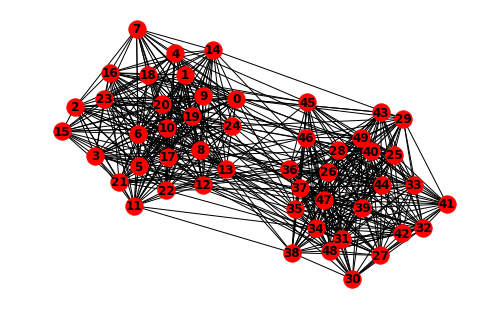
\includegraphics[scale=0.6]{static/graph_n50_pin08_pout01.png}
\caption{Graphe généré à partir des paramètres: $n=50$, $p_{in}=0.8$, $p_{out}=0.1$}
\end{figure}

L'élément discriminant du test spectral étant la variable $ \Delta p= p_{in} - p_{out}$, nous allons tester 3 valeurs représentatives des différents types de résultats:
\begin{itemize}
	\item[1-] $\Delta p \in [-1,\: 0] \implies$ le graphe ne comporte pas de structure de communauté ;
	\item[2-] $\Delta p \in [0,\: p_{lim}] \implies$ le graphe comporte une structure de communauté mais la méthode spectrale ne réussi pas à la trouver ;
	\item[2-] $\Delta p \in [p_{lim},\: 1] \implies$ le graphe comporte une structure de communauté.\\
\end{itemize}

Par la suite nous allons tester pour les valeurs $\Delta p= 0.5, 0.08, -0.5$ .
De plus nous ferons une première vague de test avec $n=100$ et une autre avec $n=1000$.
La terminologie utilisée dans les figures ci-dessous est:
\begin{itemize}
	\item[- \underline{$n,\: p_{in},\: p_{out},\: p_{lim},\: z1,\: z2$}:] sont identiques aux notations utilisées jusqu'à présent ;
	\item[- \underline{$z1\: theoric, \:z2\: theoric$}:] sont les plus grandes valeurs propres $z1$ et $z2$ calculées via les équations \eqref{z1} et \eqref{z2} ;    
	\item[- \underline{$p_{in}\: estimated, \:p_{out}\: estimated$}:] sont les probabilités du SBM calculées a posteriori grâce aux valeurs propres $z1$ et $z2$.\\
\end{itemize}
Les $p_{in}\: estimated, \:p_{out}\: estimated$ sont calculés via un calcul d'optimisation (la fonction ``fsolve'' en python).
\begin{figure}[H]
	\begin{subfigure}{.5\textwidth}
		\centering
		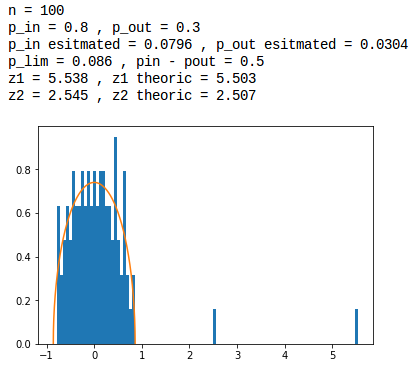
\includegraphics[scale=0.58]{static/spectral_n100_pin08_pout03.png}
		\caption{$n=100$, $\Delta p=0.5$}
		\label{n100delta05}
	\end{subfigure}
	\begin{subfigure}{.5\textwidth}
		\centering
		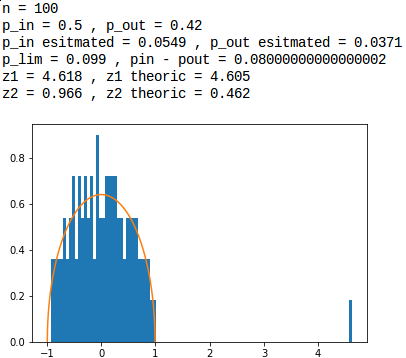
\includegraphics[scale=0.58]{static/spectral_n100_pin05_pout042.png}
		\caption{$n=100$, $\Delta p=0.08$}
		\label{n100delta008}
	\end{subfigure}
	\begin{subfigure}{.5\textwidth}
		\centering
		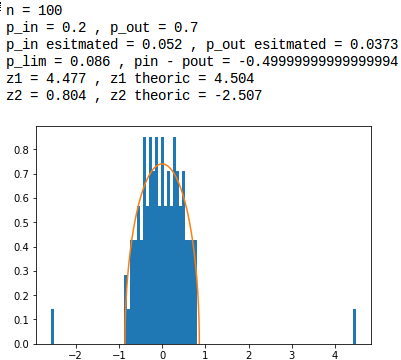
\includegraphics[scale=0.58]{static/spectral_n100_pin02_pout07.png}
		\caption{$n=100$, $\Delta p=-0.5$}
		\label{n100delta-05}
	\end{subfigure}
	\begin{subfigure}{.5\textwidth}
		\centering
		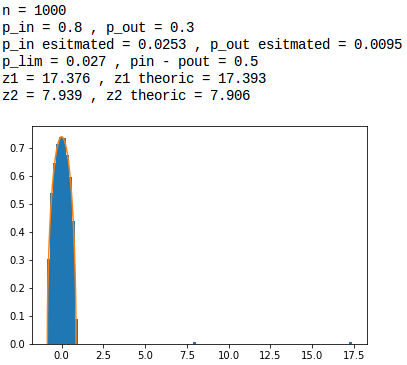
\includegraphics[scale=0.58]{static/spectral_n1000_pin08_pout03.png}
		\caption{$n=1000$, $\Delta p=0.5$}
		\label{n1000delta05}
	\end{subfigure}
	\begin{subfigure}{.5\textwidth}
		\centering
		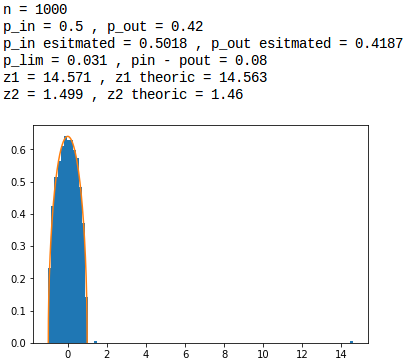
\includegraphics[scale=0.58]{static/spectral_n1000_pin05_pout042.png}
		\caption{$n=1000$, $\Delta p=0.08$}
		\label{n1000delta008}
	\end{subfigure}
	\begin{subfigure}{.5\textwidth}
		\centering
		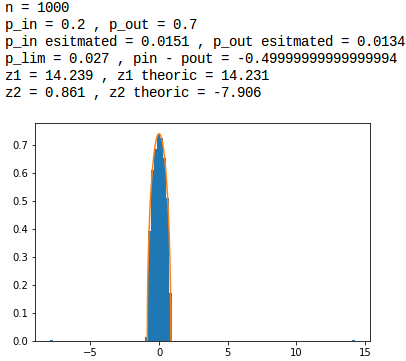
\includegraphics[scale=0.58]{static/spectral_n1000_pin02_pout07.png}
		\caption{$n=1000$, $\Delta p=-0.5$}
		\label{n1000delta-05}
	\end{subfigure}
\end{figure}

La première observation que l'on peut faire est que les valeurs propres de nos matrices d'adjacence sont bien distribuées selon la loi du demi-cercle de Wigner.
De plus, en fonction de $\Delta p$ la mesure spectrale est perturbé (ou pas) par une ou deux valeurs propres qui sortent du support de la distribution initiale.\\

Dans les cas avec $\Delta p = 0.5$ (\ref{n100delta05}, \ref{n1000delta05}), on voit très clairement deux valeurs propres qui se détachent du support de la distribution de Wigner.
Les valeurs $z1$, $z2$ correspondent bien aux valeurs théoriques et dans ce cas on retrouve, avec un taux d'erreur de l'ordre de $10^{-2}$, les valeurs $p_{in}$, $p_{out}$ du modèle utilisé pour générer le graphe.\\
Dans les cas avec $\Delta p = -0.5$ (\ref{n100delta008}, \ref{n1000delta008}), on ne s'attend pas à ce que les valeurs théorique du modèles correspondent aux valeurs trouvées par la simulation, dans la mesure où il n'y a en théorie aucune structure de communauté dans le graphe.
Cependant, on observe une valeur propre négative en dehors du support de la loi de Wigner.
Par conséquent lorsque l'on obtient une valeur propre négative, le modèle spectral nous permet de conclure qu'il n'y a pas de structure de communauté dans le graphe.\\
Enfin, dans les cas avec $\Delta p = 0.08$ (\ref{n100delta-05}, \ref{n1000delta-05}), il y a en théorie une structure de communauté. 
Cependant on se retrouve dans le cas limite décrit dans \autoref{subsec:1.3}, dans lequel le modèle ne peut en théorie pas interpréter les résultats du modèle spectral.
En effet, on peut observer qu'il n'y a qu'une seule valeur propre qui est en dehors du support, par conséquent il n'y a qu'une seule valeur propre maximale (ici $z1$) qui correspond à sa valeur théorique et de fait nous ne pouvons plus retrouver les valeurs de $p_{in}$, $p_{out}$ via les équations \eqref{z1} et \eqref{z2}.
C'est d'ailleurs confirmé par l'expérience. 

\section{Généralisation}
\subsection{Cas avec n communautés}
On peut a présent généraliser à un nombre de communautés $q \geq 2$.
Nous allons supposer que les communautés sont de même taille, à savoir $n_q = \frac{n}{q}$.
\paragraph{}\label{rq:contrainte model}
Une première contrainte apparaît, de par l'utilisation des théorèmes \ref{th:1} et \ref{th:2}, sur les valeurs des probabilités de la matrice d'adjacence $A$.
En effet, d'après le \autoref{th:1}, pour que la matrice $X$ est une mesure spectrale qui tende vers la loi de Wigner il faut que la norme 1 des vecteurs lignes de son profil de variance soient égales ($\parallel x \parallel_1 = \sum_{j=1}^{n}|x_j|$).
Par conséquent, si on veut augmenter le nombre de communautés $q$ dans le modèle, on est forcé de garder deux probabilités $p_{in}$ et $p_{out}$ qui jouent le même rôle que celles introduites précédemment (cf. \ref{rq:probability}).\\

On sait que la matrice d’adjacence du graphe sous le SBM à $q$ communautés est $A = X + \langle A \rangle$.  
Pour poursuivre l'analyse on va suivre la trame suivante:
\begin{itemize}
	\item[1-] Trouver l'équation de $\langle A \rangle$ ;
	\item[2-] Trouvez l'équation de X et déterminer son profil de variance ;
	\item[3-] Trouvez les $q$ valeurs propres associées aux perturbations de rang 1 ;
	\item[4-] Trouver $p_{lim}$.\\
\end{itemize}

% ------------------------------------------------- 1- trouver <A>  -------------------------------------------------
\subsubsection*{1- Équation de $\langle A \rangle$}
$\langle A \rangle$ étant symétrique, le théorème spectral nous dis qu'il existe une base orthonormée telle que $\langle A \rangle = \sum_{n}^{i=1}\lambda_i\mathbf{u}_i\mathbf{u}_i^{\star}$.
Après les calculs on trouve:
\begin{align} 
\langle A \rangle :&= n_q(p_{in} + (q-1)p_{out}) \mathbf{u}_1\mathbf{u}_1^{\star} + n_q(p_{in}-p_{out})\sum_{i=1}^{q-1}\mathbf{u}_i\mathbf{u}_i^{\star}\\
				   &= \frac{c_{in} + (q-1)c_{out}}{q} \mathbf{u}_1\mathbf{u}_1^{\star} + \frac{c_{in}-c_{out}}{q}\sum_{i=1}^{q-1}\mathbf{u}_i\mathbf{u}_i^{\star}
\end{align}\\
où les trois valeurs propres sont $0$, $n_q(p_{in} + (q-1)p_{out})$, $n_q(p_{in}-p_{out})$ de multiplicité $q(n_q - 1)$, $1$, $q-1$.\\

% ------------------------------------------------- 2- trouver X  -------------------------------------------------
\subsubsection*{2- Profil de variance de $\frac{X}{\sqrt{n}}$}
De la même manière que dans \autoref{ch:Analyse spectrale de la matrice d'adjacence} on trouve:
\begin{equation}
	X_{ij} \sim \left\{
	\begin{array}{lr}
		\sigma_{in} Z_{ij} & : (i,j \in P_{in}) \\
		\sigma_{out} Z_{ij} & : (i,j \in P_{out})
	\end{array}
\right.\nonumber
\end{equation}
Où $Z_{ij} = \frac{B_{ij}(p) - p}{\sqrt{p(1-p)}} \;\;avec \; p = p_{in} \; ou \; p_{out}$, $B_{ij}(p) \sim B(p)$, $B(p)$ loi de Bernoulli de paramètre p\\
La somme de n'importe quel vecteur ligne (ou colonne) du profil de variance de $\frac{X}{\sqrt{n}}$ est égale à : 
\begin{align}
\label{eq:sigma2} 
\sigma^2 = \frac{\sigma_{in}^2 + (q-1)\sigma_{out}^2}{q}
\end{align}
Le profil de variance de $\frac{X}{\sqrt{n}}$ est donc une matrice bi-stochastique.\\
% ------------------------------------------------- 3- trouver les vp -------------------------------------------------
\subsubsection*{3- Valeurs propres de $\frac{A}{\sqrt{n}}$}
Soit $\lambda$ une valeur propre de $\frac{A}{\sqrt{n}}$ et le vecteur propre associé.
\begin{align}
&\Leftrightarrow \frac{A}{\sqrt{n}}v =\lambda v \nonumber \\
&\Leftrightarrow (\Gamma - \lambda I)v =-\alpha \mathbf{11}^Tv - \beta \sum_{i=1}^{q-1}\mathbf{u}_i\mathbf{u'}_i^T \label{eq:generalize}
\end{align}
Pour trouver la valeur propre associée à $\mathbf{u}_1$ on multiplie à gauche par $\mathbf{u}_1^{\star}(\Gamma -\lambda I)^{-1}$ et on obtient:
\begin{align}
\eqref{eq:generalize} &\Leftrightarrow \mathbf{u}_1^{\star}v =-\alpha \mathbf{u}_1^{\star}(\Gamma -\lambda I)^{-1}\mathbf{u}_1\mathbf{u}_1^{\star}v - \beta \mathbf{u}_1^{\star}(\Gamma -\lambda I)^{-1}\sum_{i=1}^{q-1}\mathbf{u}_i\mathbf{u}_i^{\star}v \nonumber\\
&\xrightarrow[n \to +\infty]{} 1 = -\alpha g_{wig}^{\sigma^2}(\lambda) \nonumber\\
&\Leftrightarrow 1 = \alpha \frac{\lambda + \sqrt{\lambda^2 - 4\sigma^2}}{2\sigma^2} \nonumber\\
&\Leftrightarrow \lambda = \frac{c_{in} + (q-1)c_{out}}{q\sqrt{n}} + \frac{q\sqrt{n}\sigma^2}{c_{in} + (q-1)c_{out}} \label{eq:z_2 generalize}
\end{align}
Si on remplace $q$ par $2$ on retrouve l'équation \eqref{z_2}.\\
Pour trouver les valeurs propres associée aux $\mathbf{u}_i, \; \forall i \in \{2, \cdots, q-1\}$ on multiplie à gauche par $\mathbf{u}_2^{\star}(\Gamma -\lambda I)^{-1}$ et on obtient:
\begin{align}
\eqref{eq:generalize} &\Leftrightarrow \mathbf{u}_2^{\star}v =-\alpha \mathbf{u}_2^{\star}(\Gamma -\lambda I)^{-1}\mathbf{u}_1\mathbf{u}_1^{\star}v - \beta \mathbf{u}_2^{\star}(\Gamma -\lambda I)^{-1}\sum_{i=1}^{q-1}\mathbf{u}_i\mathbf{u}_i^{\star}v \nonumber\\
&\xrightarrow[n \to +\infty]{} 1 = -\beta g_{wig}^{\sigma^2}(\lambda) \nonumber\\
&\Leftrightarrow 1 = \beta \frac{\lambda + \sqrt{\lambda^2 - 4\sigma^2}}{2\sigma^2} \nonumber\\
&\Leftrightarrow \lambda = \frac{c_{in} - c_{out}}{q\sqrt{n}} + \frac{q\sqrt{n}\sigma^2}{c_{in} - c_{out}}\label{eq:z_1 generalize}
\end{align}
Si on remplace $q$ par $2$ on retrouve l'équation \eqref{z_1}.\\
Les valeurs propres de $A$ pour les valeurs propres de $\langle A \rangle$ égales à zéros appartiennent au support de la distribution de Wigner.
Elles n'apportent donc aucune information supplémentaire sur la structure de communauté du graphe étudié.\\   

Nous noterons $z_1 =$ \eqref{eq:z_1 generalize}  et $z_2 =$ \eqref{eq:z_2 generalize} pour la suite.
 

% ------------------------------------------------- 4- trouver p_lim -------------------------------------------------
\subsubsection*{4- Seuil de décidabilité $p_{lim}$}
Nous cherchons maintenant à déterminer $p_{lim}$.
La condition limite naturelle est celle où la valeur propre $z_2$ qui sort du support de la distribution de Wigner est égale au bord droit du support de la mesure spectrale de la matrice A.
On a alors 
\begin{align*}
	&\Leftrightarrow \lambda^+ = z_1\\
	&\Leftrightarrow 2 \sigma = \frac{c_{in} - c_{out}}{q\sqrt{n}} + \frac{q\sqrt{n}\sigma^2}{c_{in} - c_{out}}\\
	&\Leftrightarrow 0 = \beta \sigma^2 - 2 \sigma + \alpha \\
	&\Leftrightarrow p_{in} - p_{out} = \frac{q\sigma}{\sqrt{n}}  \\
\end{align*}
Donc
\begin{equation}
	p_{lim} = \frac{\sqrt{q(\sigma_{in}^2 + (q-1)\sigma_{out}^2)}}{\sqrt{n}} = \frac{q\sigma}{\sqrt{n}}  \\
\end{equation}


% ------------------------------------------------- 5- résumer -------------------------------------------------
\subsection{Bilan}
Ci-dessous le bilan de la généralisation:
\begin{align*}
	\sigma^2&: \frac{\sigma_{in}^2 + (q-1)\sigma_{out}^2}{q} \\
	z_1&: \frac{c_{in} - c_{out}}{q\sqrt{n}} + \frac{q\sqrt{n}\sigma^2}{c_{in} - c_{out}}\\
	z_2&: \frac{c_{in} + (q-1)c_{out}}{q\sqrt{n}} + \frac{q\sqrt{n}\sigma^2}{c_{in} + (q-1)c_{out}}\\
	p_{lim}&: \frac{\sqrt{q(\sigma_{in}^2 + (q-1)\sigma_{out}^2)}}{\sqrt{n}} \\
\end{align*}

% ------------------------------------------------- 6- Simulation -------------------------------------------------
\subsection{Simulations}
\begin{figure}[H]
\centering
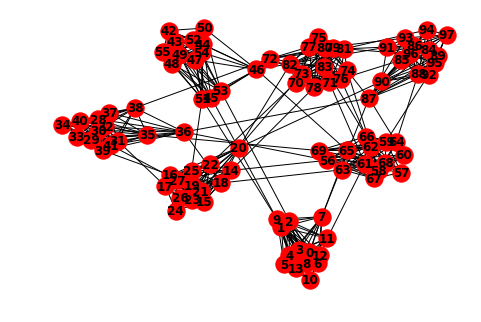
\includegraphics[scale=0.6]{static/graph_q7_n100_pin08_pout0011.png}
\caption{Graphe généré à partir des paramètres: $q=7$ $n=100$, $p_{in}=0.8$, $p_{out}=0.01$}
\end{figure}
\begin{figure}[H]
\centering
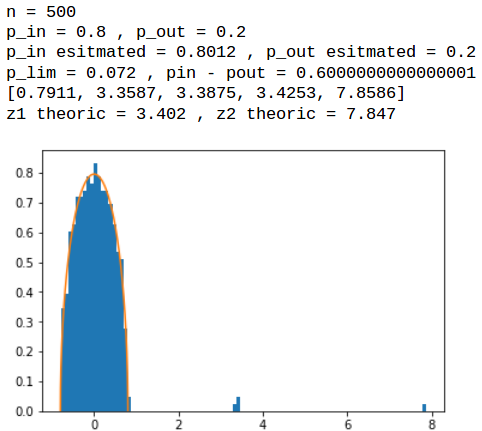
\includegraphics[scale=0.6]{static/spectral_q4_n500_pin08_pout02}
\caption{$q=4$, $n=500$, $\Delta p=0.6$}
\label{n500delta-05}
\end{figure}
\subsection{Limites du modèle}
Le première limite de ce modèle est que l'on est cantonné à des communautés de même taille $n_q$.
En effet si on change ce paramètre pour chacune des communautés alors le \autoref{th:1} n'est plus applicable, la somme des éléments de chaque vecteurs ligne du profil de variance n'est plus constant.\\

La deuxième contrainte est le fait que l'on doit toujours garder deux paramètres $p_{in}$ et $p_{out}$ indépendamment du nombre de communautés $n_q$ et du nombre de nœuds dans le graphe $n$.
Idéalement nous souhaiterions avoir un paramètre $p_{ij}$ correspondant à la probabilité d'avoir une arrête entre le nœud $i$ et le nœud $j$ et ce $\forall i<j$.\\
Une manière d'encoder ces paramètres est d'utiliser la relation suivante $p_{ij} = q_iq_jC_{\alpha}$
\begin{align}
	p_{ij} &= q_iq_jC_{g_ig_j}
\end{align}
Où $q_i$ est la probabilité intrinsèque du nœud $i$ à avoir une arrête, $g_i$ est la communauté correspondant au nœud $i$ et $C_{g_ig_j}$ est le facteur de correction par communauté.\\
Cette formalisation plus générale est très répandu dans la théorie de la détection de communauté spectrale.
\nocite{*}
\bibliographystyle{plain}
\bibliography{b}
\end{document}
